\begin{frame}[t]{Функции импульсного отклика}

\vspace{-0.25cm}

\begin{columns}[T,totalwidth=\textwidth]

\begin{column}{0.76\textwidth}
\centering
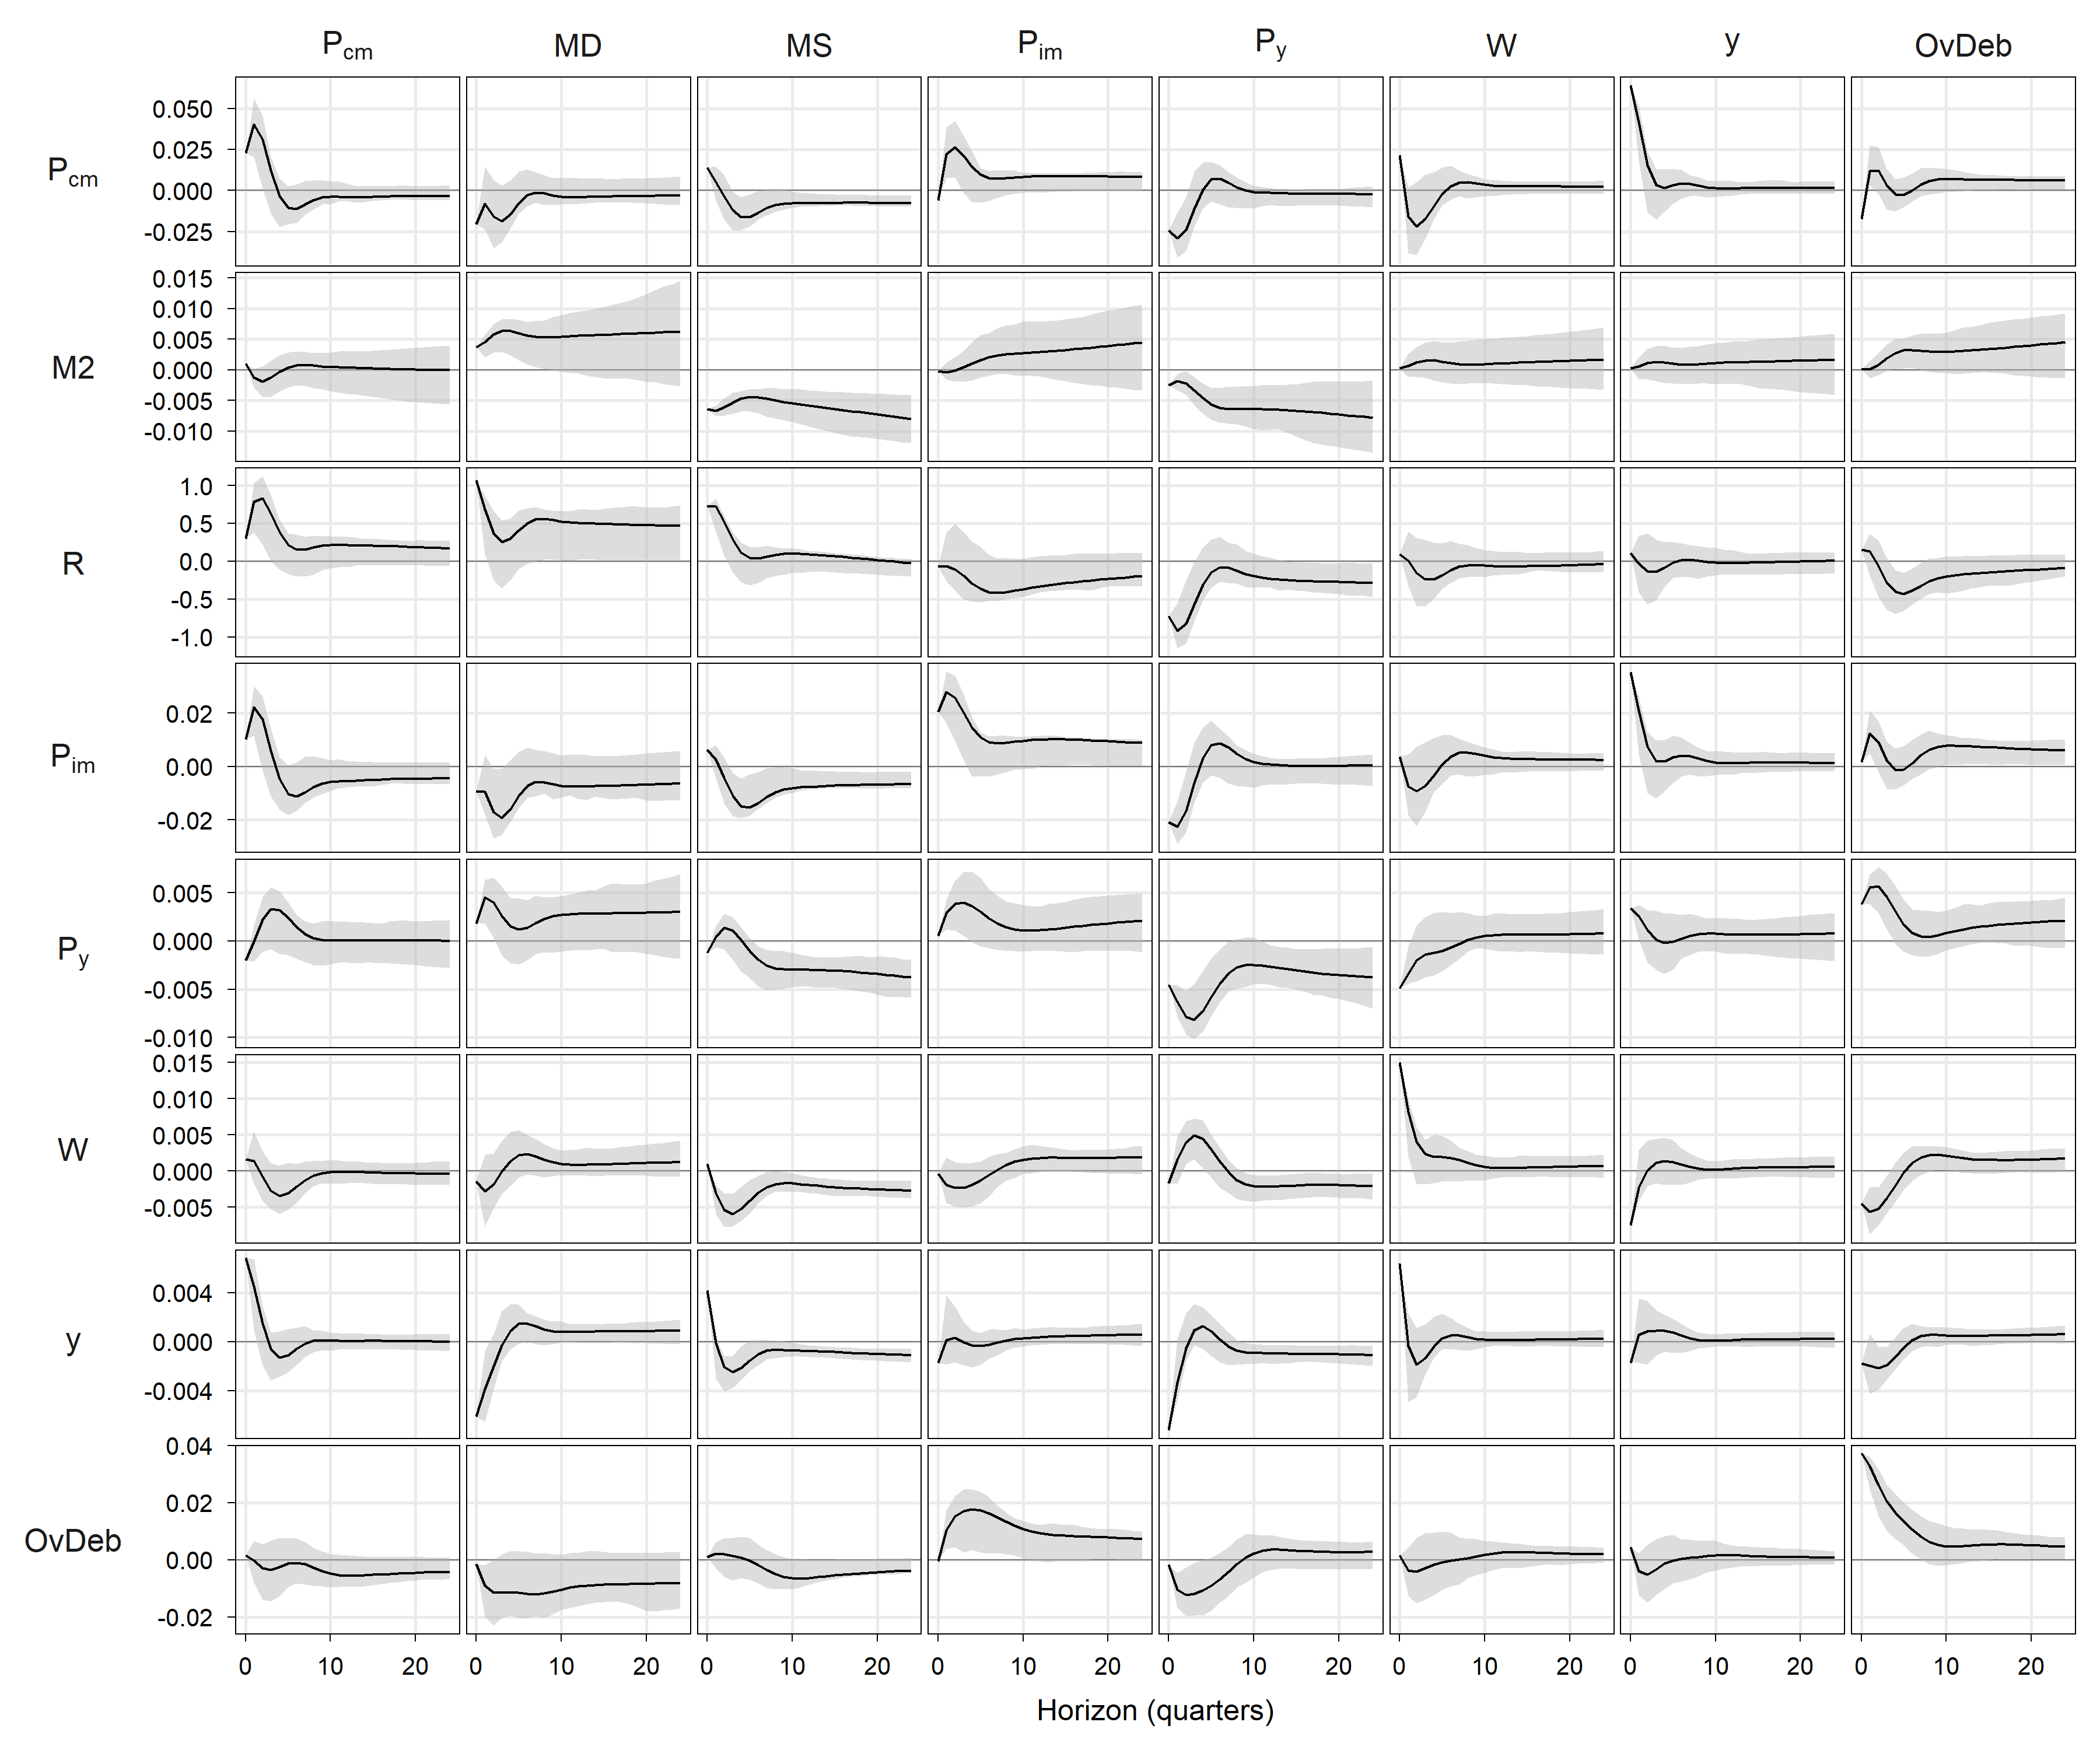
\includegraphics[
    width=\linewidth,
    height=0.84\textheight,
    keepaspectratio
]{irf_full_grid_presentation.png}
\end{column}

\begin{column}{0.22\textwidth}
\scriptsize

\textbf{Как читать график}

\vspace{0.15cm}

\begin{itemize}
    \item строки --- реагирующие переменные;
    \item столбцы --- структурные шоки;
    \item основной интерес: $MS$ и $MD$.
\end{itemize}

\vspace{0.2cm}

\textbf{Интерпретация}

\vspace{0.15cm}

Шок $MS$ соответствует ужесточению ДКП: ставка растёт, $M2$ снижается, выпуск и цены затем ослабевают.

\end{column}

\end{columns}

\end{frame}